\section{Unit Step Signal}
The unit step signal, also known as the Heaviside step function, is
0 for values less than 0 and 1 otherwise. 

\subsection{Discrete-Time Unit Step Signal}
The discrete-time unit step signal is defined as:
\[
u[n] =
\begin{cases}
1 & n \geq 0, \\
0 & n < 0.
\end{cases}
\]
Or alternatively,
\begin{equation}
    u[n] = \sum_{i = -\infty}^{n} \delta[i]
\end{equation}
In either definition, 
\[
u[n] = 1 \text{ for } n \geq 0, \text{ and } u[n] = 0 \text{ for } n < 0.
\]

Figure \ref{fig:dt unit} is the plot for the discrete-time unit step signal.
\begin{figure}[h!]
\centering
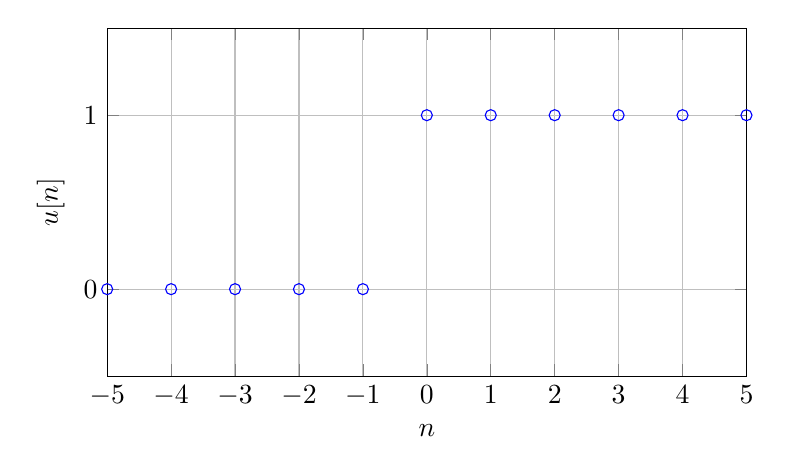
\begin{tikzpicture}
    \begin{axis}[
        xlabel={$n$},
        ylabel={$u[n]$},
        grid=major,
        ytick={0,1},
        xtick={-5,-4,...,5},
        ymin=-0.5, ymax=1.5,
        xmin=-5, xmax=5,
        width=0.8\textwidth,
        height=6cm,
        samples=100,
        domain=-5:5
    ]
    \addplot+[only marks, mark=o] coordinates {
        (-5,0) (-4,0) (-3,0) (-2,0) (-1,0)
        (0,1) (1,1) (2,1) (3,1) (4,1) (5,1)
    };
    \end{axis}
\end{tikzpicture}
\caption{Discrete-Time Unit Step Signal}
\label{fig:dt unit}
\end{figure}

A useful property for signal sampling is that, if we 
just want to consider a section of the signal between 
$0$ and $n_0$, we can just multiply $x[n]$ by $u[n] - u[n - n_0]$.

\subsection{Continuous-Time Unit Step Signal}
The continuous-time unit step signal is defined as:
\[
u(t) =
\begin{cases}
1 & t \geq 0, \\
0 & t < 0.
\end{cases}
\]
Or alternatively, 
\begin{equation}
    u(t) = \int_{-\infty}^{t} \delta(t) dt
\end{equation}

Figure \ref{fig:ct unit} is the plot for the continuous-time unit step signal:

\begin{figure}[h!]
\centering
\begin{tikzpicture}
    \begin{axis}[
        xlabel={$t$},
        ylabel={$u(t)$},
        grid=major,
        ytick={0,1},
        xmin=-5, xmax=5,
        ymin=-0.5, ymax=1.5,
        width=0.8\textwidth,
        height=6cm,
        samples=100,
        domain=-5:5
    ]
    \addplot[domain=-5:0, samples=100, thick] {0};
    \addplot[domain=0:5, samples=100, thick] {1};
    \addplot[mark=*, mark size=2pt] coordinates {(0,1)};
    \end{axis}
\end{tikzpicture}
\caption{Continuous-Time Unit Step Signal}
\label{fig:ct unit}
\end{figure}

\subsection{Discrete-Time Delta Function}
The discrete-time delta function, known as the Kronecker delta function, is defined as:
\[
\delta[n] =
\begin{cases}
1 & n = 0, \\
0 & n \neq 0.
\end{cases}
\]

Figure \ref{fig:dt delta} is the plot for the discrete-time delta function:

\begin{figure}[h!]
\centering
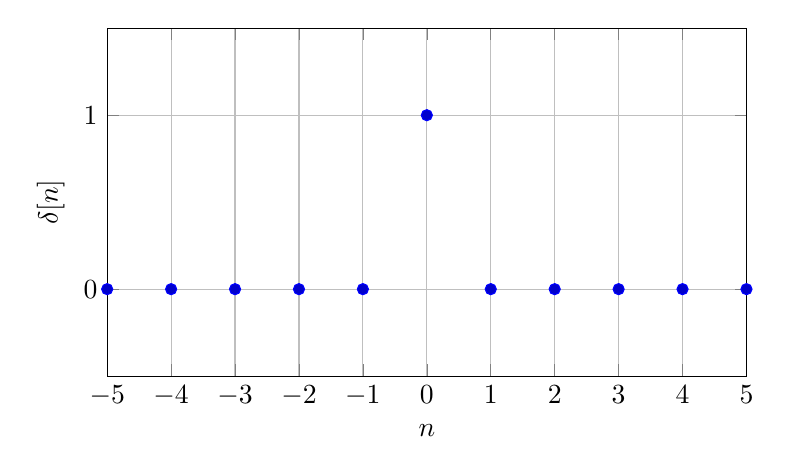
\begin{tikzpicture}
    \begin{axis}[
        xlabel={$n$},
        ylabel={$\delta[n]$},
        grid=major,
        ytick={0,1},
        xtick={-5,-4,...,5},
        ymin=-0.5, ymax=1.5,
        xmin=-5, xmax=5,
        width=0.8\textwidth,
        height=6cm,
        samples=100,
        domain=-5:5
    ]
    \addplot+[only marks, mark=*] coordinates {
        (-5,0) (-4,0) (-3,0) (-2,0) (-1,0)
        (0,1) (1,0) (2,0) (3,0) (4,0) (5,0)
    };
    \end{axis}
\end{tikzpicture}
\caption{Discrete-Time Delta Function}
\label{fig:dt delta}
\end{figure}

A useful property of the delta function in DT is that, since 
it is just equal to one when its argument is 0, then 
\begin{eqnarray}
    x[n] = \sum_{k=-\infty}^{\infty} x[k]\delta [n-k]
\end{eqnarray}

\subsection{Continuous-Time Delta Function}
The continuous-time delta function, known as the Dirac delta 
function or unit impulse, is defined as:
\[
\delta(t) = \begin{cases} 
\infty & t = 0, \\
0 & t \neq 0, 
\end{cases}
\]
with the property that:
\[
\int_{-\infty}^{\infty} \delta(t) dt = 1.
\]

An alternative definition for $\delta(t)$ is 
\begin{equation}
    \delta(t) = \frac{d}{dt} u(t)
\end{equation}

Figure \ref{fig:ct delta} is the plot for the continuous-time delta function. 
The height of the arrow indicates not the value of the function but its area, 
since the value is technically undefined. 

\begin{figure}[h!]
\centering
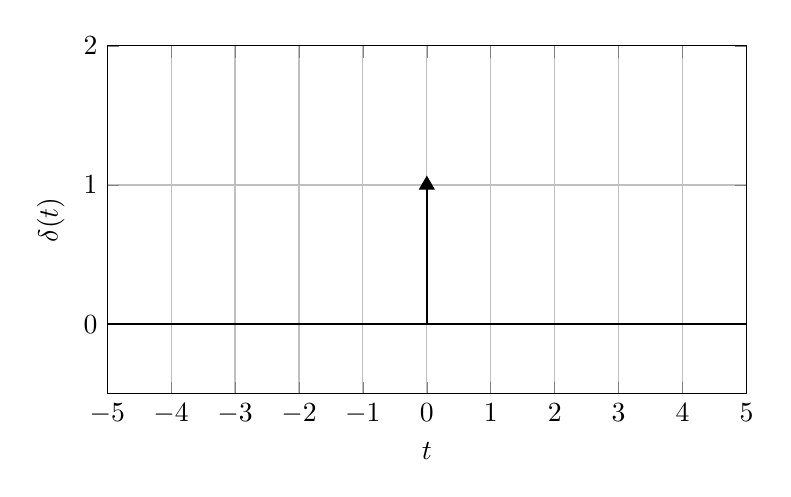
\begin{tikzpicture}
    \begin{axis}[
        xlabel={$t$},
        ylabel={$\delta(t)$},
        grid=major,
        xtick={-5,-4,-3,-2,-1,0,1,2,3,4,5},
        ymin=-0.5, ymax=2,
        xmin=-5, xmax=5,
        width=0.8\textwidth,
        height=6cm,
        samples=100
    ]
    \addplot[thick, domain=-5:5, samples=2] {0};
    \addplot[only marks, mark=triangle*, mark size=3pt] coordinates {(0,1)};
    \addplot[thick] coordinates {(0,0) (0,1)};
    \end{axis}
\end{tikzpicture}
\caption{Continuous-Time Delta Function}
\label{fig:ct delta}
\end{figure}